\section{A quantitative conjecture for the diagonal velocities}
\label{diag:q:sec}

The inverse-function identity for the diagonal branch suggests a much
sharper description of its oscillations.  This section separates the exact
local calculation from the global analytic-continuation problem that is
still open.  We restrict to the original lattice spacing $h=1$, so $A=2$.
Write
\begin{equation}\label{diag:q:inverse}
 V(t)=\sum_{n\geq1}v_n(2)t^n=\log2-u(t),\qquad
 e^{u(t)}=2+tu(t),\qquad u(0)=\log2.
\end{equation}
Thus the coefficient formula, independently of any conjecture below, is
\begin{equation}\label{diag:q:exact-coefficients}
 v_n(2)=2^{-n}\sum_{j=1}^{n}
    \stirling{n}{n-j+1}\frac{(-\log2)^j}{j!},
\end{equation}
where $\stirling{n}{k}$ denotes an unsigned Stirling number of the first kind.

\subsection{The candidate critical pair and its local expansion}
\label{diag:q:critical-subsection}

A finite critical point of the inverse relation must satisfy
\begin{equation}\label{diag:q:critical-equations}
 e^{u_*}=t_*,\qquad (1-u_*)e^{u_*}=2.
\end{equation}
We specify one conjugate pair without relying on a branch convention for
Lambert's $W$ function.  Let $\theta\in(0,\pi/2)$ be the solution of
\begin{equation}\label{diag:q:theta}
 1-\theta\cot\theta+
       \log\!\left(\frac{\theta}{\sin\theta}\right)=\log2,
\end{equation}
and put
\begin{equation}\label{diag:q:parameters}
 a=1-\theta\cot\theta,\qquad u_*=a+i\theta,\qquad
 t_*=e^{u_*},\qquad R=|t_*|=e^a.
\end{equation}
These definitions are exact.  The left side of \eqref{diag:q:theta}
increases strictly from $0$ to $1+\log(\pi/2)$, since its derivative is
\[
 \theta\csc^2\theta+\frac1\theta-2\cot\theta
 =\frac{(\theta-\sin\theta\cos\theta)^2+\sin^4\theta}
         {\theta\sin^2\theta}>0.
\]
Consequently \eqref{diag:q:theta} has exactly one solution in the stated
interval.  Direct substitution proves \eqref{diag:q:critical-equations}.
Equivalently, $u_*=1+W_0(-2/e+i0)$, using the upper boundary value of the
principal branch of Lambert's function~\cite[\S4.13]{DLMF}.

The following decimal values are numerical evaluations of the exact
definitions, not replacements for them:
\begin{align*}
 u_*&\approx0.469353635658274+1.132672497604881i,\\
 t_*&\approx0.678344933205449+1.447937273036010i,\\
 R&\approx1.598960348180173.
\end{align*}

\begin{proposition}[Exact local square-root calculation]
\label{diag:q:local}
Let $z=1-t/t_*$.  The two local inverse branches meeting at $(t_*,u_*)$
are convergent power series in $z^{1/2}$.  For the choice
\begin{equation}\label{diag:q:c}
 \chi=\sqrt{-2u_*},\qquad \Re \chi>0,\quad\Im \chi<0,
\end{equation}
one of these branches has expansion
\begin{equation}\label{diag:q:puiseux}
 u(t)=u_*+\chi z^{1/2}+b z+d_3 z^{3/2}+b_2z^2+O(z^{5/2}),
\end{equation}
where $b_2$ is a constant and
\begin{equation}\label{diag:q:b-d}
 b=\frac{u_*}{3}-1,\qquad
 d_3=\chi\left(\frac12-\frac{u_*}{18}-\frac1{4u_*}\right).
\end{equation}
The other branch changes the signs of all odd powers of $z^{1/2}$.
This statement does not identify either local branch with the germ in
\eqref{diag:q:inverse}.
\end{proposition}

\begin{proof}
Set $d=u-u_*$.  Dividing the implicit equation by $t_*$ and using
\eqref{diag:q:critical-equations} gives the exact local equation
\begin{equation}\label{diag:q:local-equation}
 e^d-1-d+z(u_*+d)=0.
\end{equation}
Equivalently,
$z=-(e^d-1-d)/(u_*+d)=-d^2/(2u_*)+O(d^3)$.
Since $u_*\neq0$, the local analytic inverse is a convergent power series
in $\sqrt z$, with its two possible signs.  Substitution of
$d=\chi z^{1/2}+b z+d_3z^{3/2}+\cdots$ into
\eqref{diag:q:local-equation} gives successively
\[
 \frac{\chi^2}{2}+u_*=0,\qquad
 \chi b+\frac{\chi^3}{6}+\chi=0,
\]
and
\[
 \chi d_3+\frac{b^2}{2}+\frac{\chi^2b}{2}+\frac{\chi^4}{24}+b=0.
\]
These identities give \eqref{diag:q:c} and \eqref{diag:q:b-d}.
\end{proof}

Numerically,
\begin{align*}
 \chi&\approx0.869892622200723-1.302083117729355i,\\
 d_3&\approx0.507703114841215-0.406328525288279i.
\end{align*}
There are infinitely many other formal critical values coming from the
other solutions of \eqref{diag:q:critical-equations}.  They have the form
$t_k=-2/W_k(-2/e)$, so the values corresponding to sufficiently remote
Lambert branches tend to zero~\cite[\S4.13]{DLMF}.
They cannot all be singularities of the germ \eqref{diag:q:inverse},
which is holomorphic near zero.  Their relevance depends on which sheet
of the inverse is reached.  Listing critical values and minimizing their
moduli therefore does not settle the radius of convergence of $V$.

\subsection{An explicit dominance conjecture and its consequence}
\label{diag:q:dominance-subsection}

\begin{conjecture}[Accessible dominant conjugate pair for $A=2$]
\label{diag:q:dominance}
For some $\epsilon>0$, the germ $u$ in \eqref{diag:q:inverse} has a
single-valued holomorphic continuation to the slit disk
\begin{equation}\label{diag:q:domain}
 \Omega_\epsilon=\{t:|t|<R+\epsilon\}
 \mathbin{\big\backslash}
 \left(
  \{s t_*:1\leq s<1+\epsilon/R\}
   \cup
  \{s\overline{t_*}:1\leq s<1+\epsilon/R\}
 \right).
\end{equation}
Its limiting values at the two slit endpoints are respectively $u_*$
and $\overline{u_*}$.  Near the upper endpoint it is the branch
\eqref{diag:q:puiseux} with $\chi$ chosen in \eqref{diag:q:c}, where
$z^{1/2}>0$ along $t=s t_*$ for $s<1$ sufficiently close to $1$.
At the lower endpoint its expansion is the complex conjugate.
\end{conjecture}

The conjecture includes three substantive claims: accessibility of the
specified critical points from the germ at zero, the identification of the
square-root sign, and absence of other singularities on or inside the
circle of radius $R$.  None is inferred here from the formal critical
equations alone.

\begin{theorem}[Conditional two-term coefficient asymptotic]
\label{diag:q:conditional-asymptotic}
Assume Conjecture~\ref{diag:q:dominance}.  Define
\begin{equation}\label{diag:q:c1}
 \chi_1=\frac{3\chi}{8}-\frac{3d_3}{2}
     =\chi\left(-\frac38+\frac{u_*}{12}+\frac3{8u_*}\right).
\end{equation}
Then the radius of convergence of $V$ is $R$, and
\begin{equation}\label{diag:q:two-term}
 v_n(2)=\frac{R^{-n}}{\sqrt\pi\,n^{3/2}}
       \Re\!\left[e^{-in\theta}
                    \left(\chi+\frac{\chi_1}{n}\right)\right]
       +O\!\left(R^{-n}n^{-7/2}\right).
\end{equation}
In particular, if $\phi=-\arg \chi$, then
\begin{equation}\label{diag:q:cosine}
 v_n(2)=\frac{|\chi|}{\sqrt\pi\,R^n n^{3/2}}
                 \cos(n\theta+\phi)
          +O\!\left(R^{-n}n^{-5/2}\right).
\end{equation}
The errors are additive; no division by the oscillating cosine is intended.
\end{theorem}

\begin{proof}
The conjectured continuation and the nonzero square-root coefficient
give radius exactly $R$.  At $t_*$ the nonintegral terms in $V=\log2-u$
are $-\chi z^{1/2}-d_3z^{3/2}$, with conjugate terms at
$\overline{t_*}$.  The exact binomial-coefficient identity and its gamma
ratio expansion give, for either nonintegral exponent used here,
\[
 [t^n](1-t/t_*)^\alpha
 =\frac{t_*^{-n}n^{-\alpha-1}}{\Gamma(-\alpha)}
   \left(1+\frac{\alpha(\alpha+1)}{2n}+O(n^{-2})\right).
\]
Using $\Gamma(-1/2)=-2\sqrt\pi$ and
$\Gamma(-3/2)=4\sqrt\pi/3$, the upper singularity contributes
\[
 \frac{t_*^{-n}}{2\sqrt\pi\,n^{3/2}}
 \left(\chi+\frac{3\chi/8-3d_3/2}{n}\right)
 +O(R^{-n}n^{-7/2}).
\]
Adding the conjugate contribution proves \eqref{diag:q:two-term}.
The slit disk contains the two dented neighborhoods needed for
singularity transfer, and the convergent Puiseux expansion supplies the
remainder estimate.  The integral powers are locally holomorphic and do
not contribute to these algebraic coefficient terms.  This is the
finite-singularity form of the transfer method of
Flajolet and Odlyzko~\cite{FlajoletOdlyzko1990}.  Taking the real part of
$\chi e^{-in\theta}$ gives \eqref{diag:q:cosine} with the stated sign.
\end{proof}

The numerical amplitude and phase are
\[
 \frac{|\chi|}{\sqrt\pi}\approx0.883480827960335,
 \qquad \theta\approx1.132672497604881,
 \qquad \phi\approx0.981817528486668,
\]
and
$\chi_1\approx-0.435344938936552+0.121211618783910i$.
Thus the conjecture predicts an exponentially decaying, algebraically
modulated oscillation.  The unconditional proof of infinitely many
positive and negative velocities does not require this conjecture.

\subsection{Exact coefficient certificates and numerical diagnostics}
\label{diag:q:diagnostics-subsection}

The accompanying script \nolinkurl{code/diagonal_quantitative.py}
evaluates \eqref{diag:q:exact-coefficients} for every integer
$50\leq n\leq200$ using exact integer interval arithmetic.  It encloses
$\log2$ by a rational truncation of
\[
 \log2=2\sum_{j=0}^{\infty}\frac1{(2j+1)3^{2j+1}},
\]
with a geometric upper bound for the tail, and evaluates the Stirling
polynomials by Horner's rule with outward rounding on a grid of size
$10^{-400}$.  Every resulting interval excludes zero; its relative width
is less than $10^{-330}$ by an exact integer comparison.  All interval
endpoints are included in \nolinkurl{data/diagonal_quantitative.json}.
An independently implemented coefficient recurrence agrees numerically
with their midpoints to over $180$ relative decimal places.

For the asymptotic comparison, put
\[
 Z_n=\sqrt\pi\,R^n n^{3/2}v_n(2),\quad
 Z_n^{(0)}=\Re(\chi e^{-in\theta}),\quad
 Z_n^{(1)}=\Re((\chi+\chi_1/n)e^{-in\theta}).
\]
The critical parameters and the model errors below were evaluated with
$280$-digit arithmetic; those model calculations are numerical, in
contrast with the exact coefficient intervals.  Normalized absolute
errors avoid spurious large relative errors near zeros of the cosine.

\begin{table}[htbp]
\centering
\small
\begin{tabular}{r r r r}
\hline
$n$ & $v_n(2)$, approximately & $|Z_n-Z_n^{(0)}|$
                                   & $|Z_n-Z_n^{(1)}|$\\
\hline
 50 & $ 7.671927522997\,10^{-14}$ & $8.4090050\,10^{-3}$ & $6.078260\,10^{-5}$\\
 75 & $-3.097444735256\,10^{-19}$ & $5.5287188\,10^{-3}$ & $2.341243\,10^{-5}$\\
100 & $ 1.476168203925\,10^{-24}$ & $4.0746493\,10^{-3}$ & $1.114101\,10^{-5}$\\
125 & $-7.660459633287\,10^{-30}$ & $3.1942636\,10^{-3}$ & $5.825053\,10^{-6}$\\
150 & $ 4.168465378193\,10^{-35}$ & $2.6016760\,10^{-3}$ & $3.133644\,10^{-6}$\\
175 & $-2.325940260211\,10^{-40}$ & $2.1739529\,10^{-3}$ & $1.629365\,10^{-6}$\\
200 & $ 1.309142927750\,10^{-45}$ & $1.8494967\,10^{-3}$ & $7.305141\,10^{-7}$\\
\hline
\end{tabular}
\caption{Diagnostic errors for the conjectured velocity asymptotic; the coefficient signs themselves have exact interval certificates.}
\label{tab:velocity-asymptotic}
\end{table}

Across all $151$ consecutive indices, the observed maxima are
\begin{align*}
 \max_{50\leq n\leq200}n|Z_n-Z_n^{(0)}|
       &\approx0.4498059481,\\
 \max_{50\leq n\leq200}n^2|Z_n-Z_n^{(1)}|
       &\approx0.4839906969.
\end{align*}
The leading model's computed sign agrees with the certified sign of
$v_n(2)$ at every tested index.  The smallest tested value of
$|Z_n^{(0)}|$ is approximately $0.0138238350$ at $n=56$; this finite
sample does not explore arbitrarily close approaches to a cosine zero.

\begin{figure}[htbp]
\centering
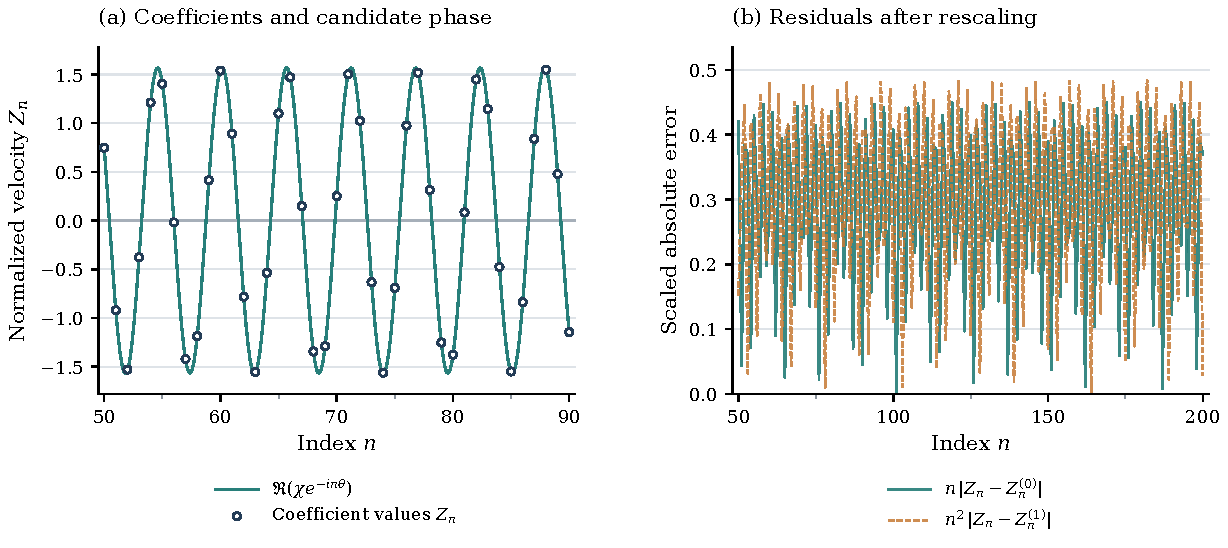
\includegraphics[width=\textwidth]{figures/diagonal_velocity_asymptotics.pdf}
\caption{Diagonal velocities and the proposed dominant conjugate pair.
Left: normalized coefficient values and the candidate oscillatory phase.
Right: leading and corrected normalized errors after multiplication
by $n$ and $n^2$. The coefficients have exact interval certificates;
the normalization and asymptotic comparison are numerical diagnostics
of Conjecture~\ref{diag:q:dominance}, not a proof of accessibility or dominance.}
\label{fig:diagonal-asymptotic}
\end{figure}

As a separate diagnostic of the local sign, the script follows the root
of \eqref{diag:q:inverse} numerically along $t=s t_*$, starting at
$u(0)=\log2$ and using successive warm Newton starts.  At the last tested
point, $1-s\approx3.76\,10^{-38}$, the estimate
$(u(s t_*)-u_*)/\sqrt{1-s}$ differs from $\chi$ by approximately
$1.8\,10^{-19}$, consistent with the next term of
\eqref{diag:q:puiseux}.  This computation was not initialized by imposing
the chosen local square-root sign.

These data support the proposed pair, local sign, and two coefficient
terms.  They do not certify continuation of a branch, prevent a numerical
root solver from changing sheets, or exclude an additional singularity of
smaller or equal modulus.  The main remaining analytic problem is to
prove or refute Conjecture~\ref{diag:q:dominance} on the inverse surface.
Even if it holds, questions about the density of positive velocities
require control of the rotation angle and of indices close to cosine
zeros; sign agreement on a finite range settles neither issue.
